\documentclass[tikz,border=8pt]{standalone}

\usetikzlibrary{arrows.meta,matrix,fit}

\newlength{\NodeSize}
\newlength{\SiblingDistance}
\newlength{\LevelDistance}
\newlength{\LabelOffset}

\setlength{\NodeSize}{6mm}
\setlength{\SiblingDistance}{6mm}
\setlength{\LevelDistance}{10mm}

\tikzset{
  tree node/.style={draw, circle, minimum size=\NodeSize, inner sep=0pt},
}

\begin{document}

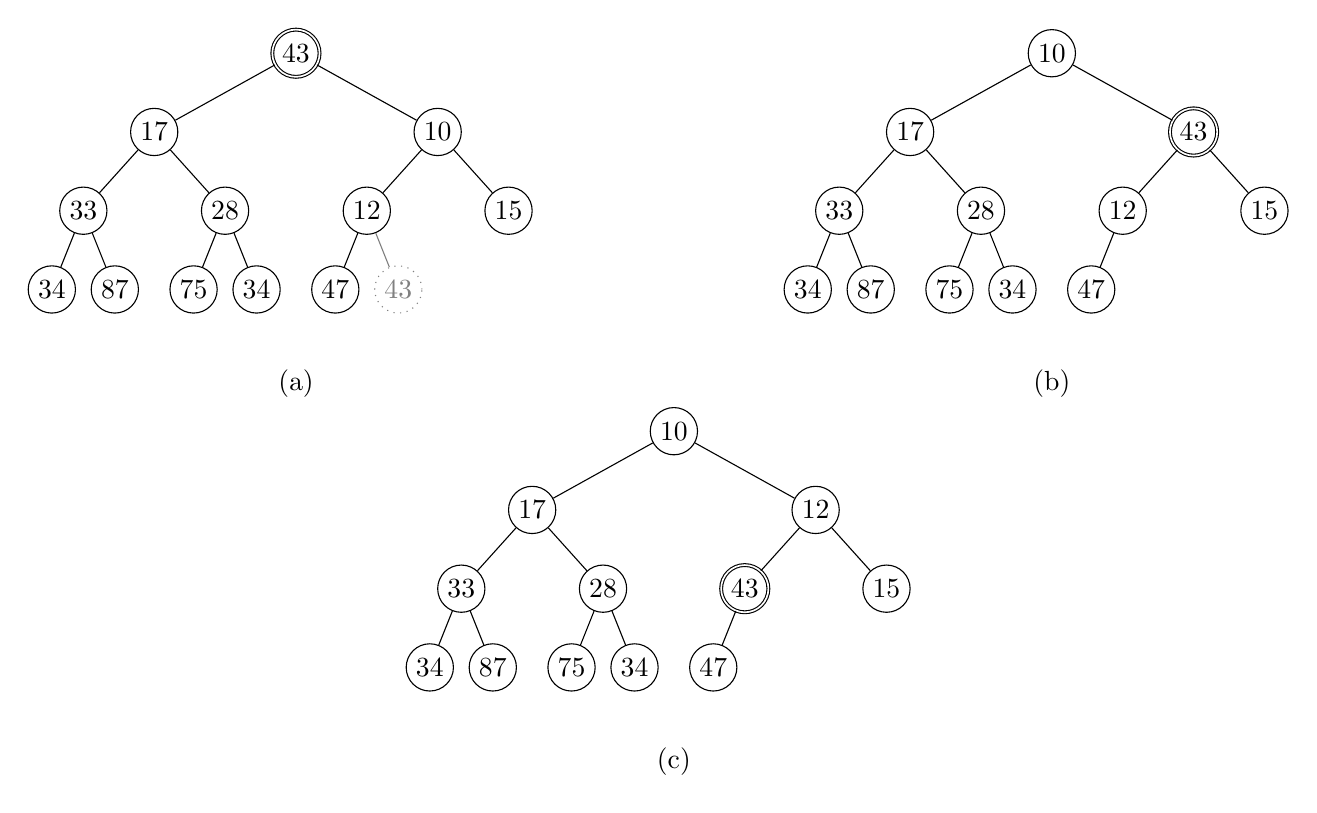
\begin{tikzpicture}[
  >=latex,
  level distance=\LevelDistance,
  level 1/.style={sibling distance=36mm},
  level 2/.style={sibling distance=18mm},
  level 3/.style={sibling distance=8mm}
]
  \begin{scope}[xshift=-48mm]
    \node[tree node, double] {43}
      child {
        node[tree node] {17}
        child {
          node[tree node] {33}
          child {node[tree node] {34}}
          child {node[tree node] {87}}
        }
        child {
          node[tree node] {28}
          child {node[tree node] {75}}
          child {node[tree node] {34}}
        }
      }
      child {
        node[tree node] {10}
        child {
          node[tree node] {12}
          child {node[tree node] {47}}
          child[edge from parent/.style={draw=gray}] {node[tree node, draw=gray, text=gray, dotted] {43}}
        }
        child {node[tree node] {15}}
      };
    \node at (0,-42mm) {(a)};
  \end{scope}

  \begin{scope}[xshift=48mm]
    \node[tree node] {10}
      child {
        node[tree node] {17}
        child {
          node[tree node] {33}
          child {node[tree node] {34}}
          child {node[tree node] {87}}
        }
        child {
          node[tree node] {28}
          child {node[tree node] {75}}
          child {node[tree node] {34}}
        }
      }
      child {
        node[tree node, double] {43}
        child {
          node[tree node] {12}
          child {node[tree node] {47}}
          child[missing] 
        }
        child {node[tree node] {15}}
      };
    \node at (0,-42mm) {(b)};
  \end{scope}

  \begin{scope}[yshift=-48mm]
    \node[tree node] {10}
      child {
        node[tree node] {17}
        child {
          node[tree node] {33}
          child {node[tree node] {34}}
          child {node[tree node] {87}}
        }
        child {
          node[tree node] {28}
          child {node[tree node] {75}}
          child {node[tree node] {34}}
        }
      }
      child {
        node[tree node] {12}
        child {
          node[tree node, double] {43}
          child {node[tree node] {47}}
          child[missing] 
        }
        child {node[tree node] {15}}
      };
    \node at (0,-42mm) {(c)};
  \end{scope}
\end{tikzpicture}





\end{document}
